\chapter{Grundlagen von elliptischen Kurven}

\section{Begriffsabgrenzung}


Nach Dietmer ist unter dem Begriff  \textbf{Kryptographie} \enquote{die Wissenschaft von geheimen Schreiben zu verstehen.} Grundkonzept eines kryptografischen Systems ist also die Verschlüsselung von Informationen bzw. von Daten, um die Vertraulichkeit der Informationen zu gewährleisten \cite{damer}.

Daten, die über einen unsicheren Kanal wie das Internet übertragen werden, werden mit Hilfe moderner Kryptosysteme so verschlüsselt, dass Unbefugte in einem Szenario, in dem sie auf die Informationen zugegriffen haben, diese nicht frei lesen und verstehen können \cite{moVarol}. \\
Die unverschlüsselte Information wird als \textit{Klartext} (Plaintext, Cleartext), die Verschlüsselte als \textit{Chiffretext} (Ciphertext, Cryptotext) bezeichnet und der Verschlüsselungsprozess des Klartextes wird \textit{chiffrieren} (engl. encryption) genannt. Umgekehrt wird unter \textit{dechriffrieren} (engl. decryption), der Entschlüsselungsprozess eines Chiffretextes, verstanden.

Im Allgemeinen werden die beiden Prozesse durch eine Reihe von Regeln erreicht, sogenannte Verschlüsselungs- und Entschlüsselungsalgorithmen. Der Verschlüsselungsprozess basiert auf einem Schlüssel, der dann zusammen mit den Informationen als Eingabe an einen Verschlüsselungsalgorithmus übergeben wird. 
Danach können unter Verwendung eines Entschlüsselungsalgorithmus die Informationen mit dem entsprechenden Schlüssel abgerufen werden. Wer einen geheimen Schlüssel besitzt, kann die Informationen in Klartext entschlüsseln \cite{moVarol}. Die folgende Abbildung \ref{konzept} verdeutlicht die Zusammenhänge.

\begin{figure}
    \centering
    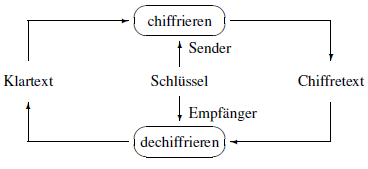
\includegraphics[width = 0.5 \textwidth]{Graphics/Cipher.png}
    \caption{Grundkonzept der Kryptographie}
    \label{konzept}
\end{figure}


In den 70er und 80er Jahren war die Kryptographie vor allem auf dem militären und diplomatischen Sektor beschränkt. Um geheime Nachrichten zu verschlüsseln, wurden sogenannte symmetrische Verschlüsselungsverfahren (z.B. Caesar-Verschlüsselung (\cite{moVarol})) verwendet, wo nur ein gemeinsamer geheimer Schlüssel sowohl für die Ver- als auch für die Entschlüsselung benutzt wird.\\

Aus diesem Grund ist es bei der symmetrischen Verschlüsselung sehr wichtig, dass der geheime Schlüssel auf einem sicheren Übertragungsweg an den Empfänger weitervermittelt wird, bevor die verschlüsselten Nachrichten übermittelt werden können. Früher wurde der Schlüssel meist persönlich, in Form eines Botens, übergeben. 
Da das persönliche Übergeben des Schlüssels sehr umständlich ist und das Risiko besteht, dass der Schlüssel belauscht oder gestohlen werden könnte, wurden weitere Verschlüsselungsverfahren vorgeschlagen. Dies sind die asymmetrischen Verschlüsselungsverfahren (auch Public-Key-Verfahren genannt) \cite{werner}. 

Im Gegensatz zu einem symmetrischen Verschlüsselungsverfahren erfordern asymmetrische Verschlüsselungsverfahren, nicht nur einen Schlüssel, sondern ein Schlüsselpaar bestehend aus einem öffentlichen Schlüssel und einem privaten Schlüssel \cite{damer}. Die Kommunikation erfolgt hier ohne vorhergehenden Schlüsselaustausch und ist jedoch viel langsamer als die Kryptografie mit privaten Schlüsseln. Mit dem privaten Schlüssel werden Daten entschlüsselt oder digitale Signaturen erzeugt, während mit dem öffentlichen Schlüssel Daten verschlüsselt und die Authentizität von erzeugten Signaturen überprüft  werden (\cite{sahuMa}; \cite{damer}). Die Abbildung \ref{key} veranschaulicht diese Schlüssel. 

\begin{figure}[!htb]
    \centering
    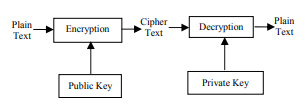
\includegraphics[width = 0.5 \textwidth]{Graphics/Fig1Encryption.png}
    \caption{Public-Key Verschlüsselung}
    \label{key}
\end{figure}


Das erste asymmetrische Kryptosystem, Rivest-Shamir-Adleman-Verfahren (RSA-Verfahren) wurde im Jahr 1977 von Ronald Rivest, Adi Shamir und Leonard Adleman gefunden, 
danach wurden weitere Kryptosysteme wie Rabin, Elgamal und Elliptische Kurven-Kryptogrphie vorgestellt.\\
Für unsere Arbeit liegt jedoch der Schwerpunkt auf der Kryptographie mit elliptischen Kurven und die Erzeugung von Schlüsseln, die für das Diffie-Hellman-Verfahren notwendig sind.\\

Die \textbf{elliptische Kurven-Kryptographie (ECC)} ist eine Verschlüsselungstechnik mit öffentlichem Schlüssel, 
die auf der algebraischen Struktur elliptischer Kurven über endlichen Körper basiert \cite{mihNita} und zur Erstellung schnellerer, kleinerer und effizienterer kryptografischer Schlüssel verwendet werden kann \cite{khan}.\\

Die Verwendung einer elliptischen Kurve in der Kryptographie wurde im Jahr 1985 unabhängig voneinander von Miller \cite{miller} und Koblitz \cite{koblitz} vorgeschlagen. In den späten 1990er Jahren wurde ECC von einer Reihe von Organisationen wie ANSI \cite{ansi}, IEEE \cite{ieee}, ISO \cite{iso}, NIST \cite{nist} standardisiert und erhielt kommerzielle Akzeptanz \cite{GaMoDa}.
Das bekannteste Verschlüsselungsschema ist das Elliptic Curve Integrated Encryption Scheme (ECIES), das in IEEE- und auch in SECG SEC 1-Standards enthalten ist \cite{marKaur}. Beispiele für die Anwendung von ECC sind unter anderen Mehrzweck-Smartcards wie die  neuen  deutschen  Ausweisdokumente \cite{merLo}.\\

Außerdem basieren Kryptosysteme mit öffentlichem Schlüssel auf der Lösung bestimmter mathematischen Probleme, z.B. beruht das RSA-Verfahren auf dem Integer Faktorisierungsproblem, DH und ECC basieren auf dem Diskreten Logarithmus-Problem. Bei der Lösung dieser Probleme stellt man im direkten Vergleich jedoch fest, dass herkömmliche Kryptosysteme mit öffentlichen Schlüsseln wie RSA Nachteile aufweisen.

Das Hauptproblem besteht darin, dass die Schlüsselgröße ausreichend groß sein muss, um die Sicherheitsanforderungen auf hohem Niveau zu erfüllen, was zu einer geringeren Geschwindigkeit und einem höheren Bandbreitenverbrauch führt.\\

Dies ist nicht den Fall, wenn elliptische Kurven (EC) für das Public Key Verfahren eingesetzt sind, da ECC im Vergleich zu RSA für den Benutzer eine gleichwertige Sicherheit bei kleineren Schlüsselgrößen bietet und für Angreifer schwere exponentielle Zeitherausforderung, um in das System einzudringen \cite{GaMoDa}.\\

Laut einigen Forschern kann ECC mit einem 164-Bit-Schlüssel ein Sicherheitsniveau erreichen, für dessen Erreichung andere Systeme einen 1.024-Bit-Schlüssel benötigen \cite{khan}. Es stellte sich heraus, dass ECC das effizienteste Kryptosystem mit öffentlichem Schlüssel ist \cite{naRaj}.
Der Grund dafür ist, dass nach Miller und Koblitz das Diskreter-Logarithmus-Problem für elliptische Kurven schwerer sei, als das klassische Diskreter-Logarithmus-Problem ist und zudem auch schnellere Laufzeiten ermögliche.\\
Bevor das Diskreter-Logarithmus-Problem vorgestellt wird, ist es wichtig zu definieren, was unter einer elliptischen Kurven zu verstehen ist. 

Im Allgemeinen ist eine elliptische Kurve eine projektive, algebraische Kurve \textbf{C(K)}, auf der sich ein bestimmter Punkt O befindet, der als Punkt unendlich oder Nullpunkt bezeichnet wird \cite{GaMoDa}.\\

Eine \textbf{elliptische Kurve E} über ein Körper $ K $ der Charakteristik $ \neq $
2 oder 3, lässt sich formal definieren als die Menge der Punkte
$ (x, y) $ $ \in $ \( K \)  der Weierstraß-Gleichung:

\begin{ceqn}

\begin{equation}
       y^2 = x^3 + ax + b \quad 
       \text{ mit a, b $ \in $ $ K $           \cite{koblitz}.}
\end{equation} 

\end{ceqn}

Elliptische Kurven in Form von Gleichungen können in \textbf{singuläre} und \textbf{nicht-singuläre} Gruppen unterteilt werden. In der ECC werden nicht-singuläre Kurven bevorzugt, damit eine Kurve frei von Spitzen oder Selbstüberschneidungen ist \cite{razad}.\\

Eine elliptische Kurve wird als \textbf{nicht-singulär} bezeichnet,
wenn sie keinen Punkt $ P = (x, y) $ enthält, an dem ein
mathematisches Objekt nicht definiert ist \cite{werner} und für
die Werte a und b folgende Bedingung $ \Delta = 4a + 27b \neq 0
$ erfüllt, um eine endliche Abelsche Gruppe zu bilden.\\

In der abstrakten Algebra ist eine \textbf{abelsche} bzw. eine
\textbf{kommutative} Gruppe, eine Gruppe \textit{G}, in der das
Ergebnis der Anwendung der Gruppenoperation auf zwei
Gruppenelemente nicht von ihrer Reihenfolge abhängt. Also wenn \(a \cdot b = b \cdot a\) \quad \(\forall a, b \in \textit{G}\), wobei \(\glqq \cdot \grqq{}\) eine Verknüpfung auf $\textit{G}$.\\

Ein \textbf{Körper} ist eine Menge \textit{K} mit zwei
Verknüpfungen \((\glqq + \grqq{},\glqq \cdot \grqq)\), sodass gilt:
\begin{enumerate}
    \item \((\textit{K}, +)\) ist eine abelsche Gruppe. Das neutrale
    Element wird mit 0 und das inverse von \(a \in \textit{K}\)  mit -a bezeichnet, 
    \item \((\textit{K}\setminus 0, \cdot)\) ist eine abelsche Gruppe mit neutralem Element 1 und $ a^{-1} $ als inversem Element zu \(a \in \textit{K}\).
    \item Distributivgesetze:
    \begin{ceqn}
     \begin{align*}
          a \cdot (b + c ) = (a \cdot b) + (a \cdot c) \quad \forall a, b, c \in \textit{K} \\
         (a + b) \cdot c = (a \cdot c) + (a \cdot b) \quad \forall a, b, c \in \textit{K}
     \end{align*}
    \end{ceqn}
    
\end{enumerate} 
Ein Körper mit endlich vielen Elementen heißt endlicher Körper. Ein solcher Körper mit p Elementen wird mit $ \mathbf{F_p}$ (auch:
$ \mathbf{GF(p)} $) bezeichnet.\\

Die \textbf{Charakteristik} eines Körpers $ \mathbf{K} $ ist die kleinste positive Zahl \textbf{p} mit 
\begin{ceqn}
\begin{align*}
   \underbrace{1 \cdot 1 \cdot 1 \cdot \ldots \cdot 1}_{\text{$k$ mal} } = 0   \quad \text{, falls sie existiert.}
\end{align*}
\end{ceqn}
 
Dies ist beispielsweise für die Körper der rationalen Zahlen $ \mathbb{Q} $, der reelen Zahlen $ \mathbb{R} $ und der komplexen Zahlen $\mathbb{C} $ der Fall. Für jeden endlichen Körper ist die Charakteristik immer eine Primzahl \cite{damer}.

$ \mathbf{K} $ kann ein beliebiger Körper, also etwa $ \mathbb{R} $, $ \mathbb{Q} $, $ \mathbb{C} $ oder ein endlicher Körper $ \mathbb{F} $ sein \cite{werner}. Die obige Gleichung entspricht der Definition einer elliptischen Kurve über reelen Zahlen.\\

Obwohl eine elliptische Kurve über die reellen Zahlen ein guter Ansatz ist, um die Eigenschaften einer elliptischen Kurve zu verstehen, erfordert sie eine höhere Rechenzeit, um verschiedene Operationen auszuführen. Sie ist manchmal aufgrund von Rundungsfehlern ungenau. Kryptographie-Schemata erfordern jedoch eine schnelle und präzise Arithmetik \cite{razad}. Folglich werden in kryptografischen Anwendungen zwei Arten von elliptischen Kurven verwendet:
	\begin{itemize}
	    \item Primzahlen über einem Feld $ \mathbf{Z_p} $, wobei p eine Primzahl und p > 3 ist. Alle Variablen und Koeffizienten werden aus einer Menge von ganzen Zahlen von 0 bis p - 1 entnommen und Berechnungen werden über Modulo p durchgeführt \cite{werner}.
        \item 	Binäre Kurve über dem Galois-Feld $ 2^m $, auch bekannt als $ GF(2^m) $, wobei alle Variablen und Koeffizienten in $ GF $ sind und Berechnungen über $ GF(2^m) $ durchgeführt werden.
	\end{itemize}

Da Primkurven analog zur Binärkurve keine erweiterte Bit-Fidding-Operation haben, sind sie für die Software-Implementierung geeignet \cite{razad}.\\



In dieser Arbeit wurde die Implementierung von elliptischen Kurven über endliche Körper mit $ \mathbf{K} $ = $ \mathbf{Z_p} $ berücksichtigt. Dazu wird in Kapitel 4 mehr erläutert.
Eine elliptische Kurve über dem endlichen Feld $ \mathbf{Z_p} $ enthält alle Punkte $ (x, y) $ in der $ \mathbf{Z_p} $ $ \times $ $ \mathbf{Z_p} $ Matrix, die die folgende elliptische Kurvengleichung erfüllt: 

\begin{ceqn}

\begin{equation}
     y^2 = x^3 + ax + b  \quad \pmod p
     \label{curve}
\end{equation}

\end{ceqn}

Dabei sind x und y Zahlen in $ \mathbf{Z_p} $  und ähnlich wie im realen Fall ist $ \Delta \neq $ 0.
Alle Punkte $ (x, y) $, die die obige Gleichung  erfüllen, liegen auch auf der elliptischen Kurve. Der öffentliche Schlüssel ist ein Punkt auf der Kurve und der private Schlüssel ist eine Zufallszahl. Das Hinzufügen von Punkten auf der elliptischen Kurve ist jedoch kein einfacher Prozess, sondern an ein in Polynomialzeit zu lösendes Problem gebunden \cite{mo2014}: Das diskrete Logarithmusproblem. 


\section{Diskretes Logarithmusproblem }

Bevor das Problem des diskreten Logarithmus erläutert wird, muss noch der Begriff der zyklischen Gruppe erklärt werden.\\ 

Eine \textbf{zyklische Gruppe} ist eine Gruppe, deren Elemente
als Potenz eines ihrer Elemente dargestellt werden können. Also wenn es ein \(a \in \textit{G}\) gibt mit \(\langle a \rangle = G\).\\ 

Nehmen wir nun an, dass (G, $ \times $ ) eine multiplikative zyklische Gruppe mit Domainparametern g, h und n ist.   
Das \textbf{diskrete Logarithmusproblem} ist explizit definiert, als das Problem der Bestimmung einer eindeutigen Ganzzahl $ x $, die zufällig aus dem Intervall [1, p - 1] ausgewählt wird, so dass gilt:
\begin{ceqn}

\begin{align*}
                g^x = h \mod p
\end{align*}

\end{ceqn}
vorausgesetzt, dass eine solche ganze Zahl existiert.
Der Parameter $ g $ ist die Basis des Logarithmus bzw. ein Erzeuger der Gruppe $ \mathbf{G} $ ; $ n $ die Anzahl der Elemente in $ \mathbf{G} $ ; der private Schlüssel bzw. das diskrete Logarithmusproblem von $ h $ zur Basis $ g $  ist die Ganzzahl $ x $, und der öffentliche Schlüssel ist   $ h = g^x $ \cite{Hankerson}. \\


Das \textbf{Elliptic Curve Diskrete Logarithmus Problem (ECDLP)} ist ähnlich definiert, aber betrachtet die Weierstraß-Gleichung für eine elliptische Kurve $ \mathbf{E:} $ $ y^2 = x^3 + ax + b $ über $ \mathbb{Z_p} $ und zwei Punkte $ P $ und $ Q $ $\in $ $ \mathbf{F_p} $.  Zu bestimmen ist, eine Zahl k $ \in $ $ \mathbf{Z} $ mit

\begin{ceqn}
\begin{align*}
      Q = kP  \quad \text{, falls so ein k existiert.}
\end{align*}
   
\end{ceqn}

Die Primzahl p, die Gleichung der elliptischen Kurve E und der Punkt P und seine Ordnung n sind die Domainparameter. Der private Schlüssel ist die ganze Zahl k, die gleichmäßig zufällig aus dem Intervall [1, n - 1] ausgewählt wird, und der entsprechende öffentliche Schlüssel ist $ Q = kP $.

Daher ist die Hauptoperation bei der ECC die Punktmultiplikation, also die Multiplikation eines Skalars k mit einem beliebigen Punkt P auf der Kurve, um einen anderen Punkt Q auf der Kurve zu erhalten. 

Das Lösen von ECDLP ist viel schwieriger als DLP, da die Komplexität der Punktarithmetik in ECDLP im Vergleich zur Ganzzahlarithmetik in DLP zunimmt. 
Aus diesem Grund ist ECC in der Lage, ein ähnliches Sicherheitsniveau wie RSA bereitzustellen, jedoch mit einer kürzeren Schlüsselgröße, was es wiederum zur beliebtesten Wahl macht \cite{mo2014}.\\ 

Damit ein auf $ \mathbf{F_p} $ basierendes diskretes Logarithmus-System effizient ist, sollten schnelle Algorithmen zur Berechnung der Gruppenoperation bekannt sein. Aus Sicherheitsgründen sollte das Problem des diskreten Logarithmus in $ \mathbf{Z_p} $ unlösbar sein \cite{Hankerson}. \\
Es gibt viele Algorithmen zur Lösung von \textbf{ECDLP}, aber der erfolgreichste ist die Kombination von Pollards Rho- und Pohlig-Hellman-Angriffen mit vollständig exponentieller Laufzeit (\cite{mo2014};\cite{Hankerson}). 
Angriffe resultieren normalerweise aus den Schwächen bei der Auswahl der elliptischen Kurve und des endlichen Feldes (siehe Kapitel 4 und 5), aber die meisten Angriffe können durch korrekte Auswahl der Parameter der elliptischen Kurve vereitelt werden \cite{mo2014}.
Daher sollten diese öffentlichen Parameter sicher ausgewählt werden, um alle bekannten Angriffe zu vermeiden \cite{aliKa}. Der nächste Abschnitt beschäftigt sich näher mit diesen Parametern. 

\section{Domänenparameter für elliptischen Kurven}

Vor der Implementierung eines ECC-Systems müssen mehrere Entscheidungen getroffen werden.
Dazu gehören die Auswahl von Domänenparametern für elliptische Kurven (zugrunde liegendes endliches Feld, Felddarstellung, elliptische Kurve) sowie Algorithmen für Feldarithmetik, elliptische Kurvenarithmetik und Protokollarithmetik.\\

Die Auswahl kann durch Sicherheitsaspekte, Anwendungsplattform (Software oder Hardware), Einschränkungen der jeweiligen Computer- und Kommunikationsumgebung (z. B. Speichergröße, Bandbreite) beeinflusst werden \cite{Havaze}.\\

Bevor der Verschlüsselungsprozess gestartet und der verschlüsselte Text transformiert wird, müssen Domänenparameter von beiden
Parteien vereinbart werden, die an der sicheren und vertrauenswürdigen Kommunikation über ECC beteiligt sind \cite{sosax}.
Sie werden von einer Gruppe von Benutzern gemeinsam genutzt und können in einigen Anwendungen jedoch für jeden Benutzer spezifisch sein \cite{kalsa}.
Es können zwei Arten von elliptischen Kurvendomänenparametern verwendet werden \cite{standard}:
\begin{itemize}
    \item elliptische Kurvendomänenparameter über $ \mathbf{Z_p} $ und
    \item elliptische Kurvendomänenparameter über $ \mathbf{F_2^m} $ .
\end{itemize}

\subsection{Parameter über \texorpdfstring $ \mathbf{ Z_p } $ }

Die Domänenparameter für die elliptische Kurve über $ \mathbf{F_p} $ sind  ein Sextuple
\begin{ceqn}
\begin{align*}
  (p, a, b, G, n, h)  
\end{align*}
\end{ceqn}
 bestehend aus einer ganzen Zahl $ \mathbf{ p } $, die das endliche Feld $ \mathbf{ Z_p} $ spezifiziert; der Kurve aus \ref {curve}, den Parametern a und b, einem Basispunkt $  G = (x_G, y_G) $ auf $ E(\mathbf{Z_p}) $,  $ \mathbf{ n } $ die Ordnung der elliptischen Kurve und dem Cofaktor h, wobei 
 \begin{ceqn}
 \begin{align*}
   h = \frac{ \#E ({F_p}) }{ n } 
 \end{align*} 
 \end{ceqn}
und $ \#E (\mathbf{F_p}) $  die Anzahl der Punkte auf einer elliptischen Kurve ist (\cite{standard}; \cite{GaMoDa}).\\


\subsection{Parameter über \texorpdfstring $ \mathbf{F_2^m} $}

Die Domänenparameter für die elliptische Kurve über $ \mathbf{ F_2^m } $ sind ein Septuple
\begin{ceqn}
\begin{align*}
           T = (m, f (x), a; b; G; n; h) 
\end{align*}
\end{ceqn}
bestehend aus einer ganzen Zahl $ m $, einem irreduziblen binären Polynom $ f (x) $ vom Grad m, Parameter a, b $ \in $ $ \mathbf{ F_2^m} $ der durch die Gleichung der elliptischen Kurve $ \mathbf{ E (F_2^m)} $:
\begin{ceqn}
\begin{equation}
           y^2 + xy = x^3 + ax^2 + b  \quad \in F_2^m
\end{equation}
\end{ceqn}
definiert sind, einem Basispunkt $ G = (xG; yG) $ auf $ E (F_2^m) $, eine Primzahl n, die in der Größenordnung von G liegt und die Cofaktor h mit 
\begin{ceqn}
 \begin{align*}
   h = \frac{ \#E ({F_p}) }{ n } 
 \end{align*} 
 \end{ceqn}
und $ \#E (\mathbf{F_p}) $  die Anzahl der Punkte auf einer elliptischen Kurve ist. (\cite{standard}; \cite{GaMoDa})


Um einen Angriff auf ECDLP zu vermeiden, muss $ |E| $ eine ausreichend große Primzahl sein. Zumindest wird vorgeschlagen, dass $ n > 2^{160} $ ist \cite{kalsa}.\\


Für diese Arbeit wurden Parameter in $ \mathbf{ Z_p } $ bevorzugt. 
Die Verwendung der elliptischen Kurvenarithmetik macht ECC unter allen vorhandenen kryptografischen Schemata einzigartig.
Je nach gewähltem Feld verwendet ECC für seine Operationen modulare Arithmetik oder Polynomarithmetik. Dies wird im nächsten Kapitel präsentiert. 


